\documentclass{article}
\usepackage{tikz}
\usepackage{tkz-euclide}
\usepackage{pgfplots}
\usepackage{fancyhdr}

\usepackage{graphicx}
\usetikzlibrary{arrows.meta}
\pagestyle{fancy}
\fancyhf{} % Clear all header and footer fields
\fancyhead[L]{Your Name} % Left header with name
\fancyhead[R]{Septermber 14th 2025} % Right header with date
\begin{document}
\section{Graph 1}

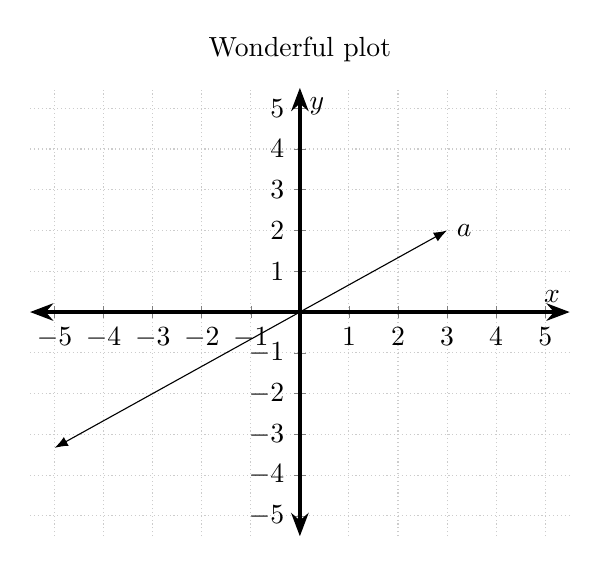
\begin{tikzpicture}
\begin{axis}[
  axis lines=middle,
  axis line style={Stealth-Stealth,very thick},
  xmin=-5.5,xmax=5.5,ymin=-5.5,ymax=5.5,
  xtick distance=1,
  ytick distance=1,
  xlabel=$x$,
  ylabel=$y$,
  title={Wonderful plot},
  grid=major,
  grid style={thin,densely dotted,black!20}]
\addplot [Latex-Latex,domain=-5:3,samples=2] {x*2/3} node[right]{$a$};
\end{axis}
\end{tikzpicture}

\vspace{1cm}
\section{Graph 2}

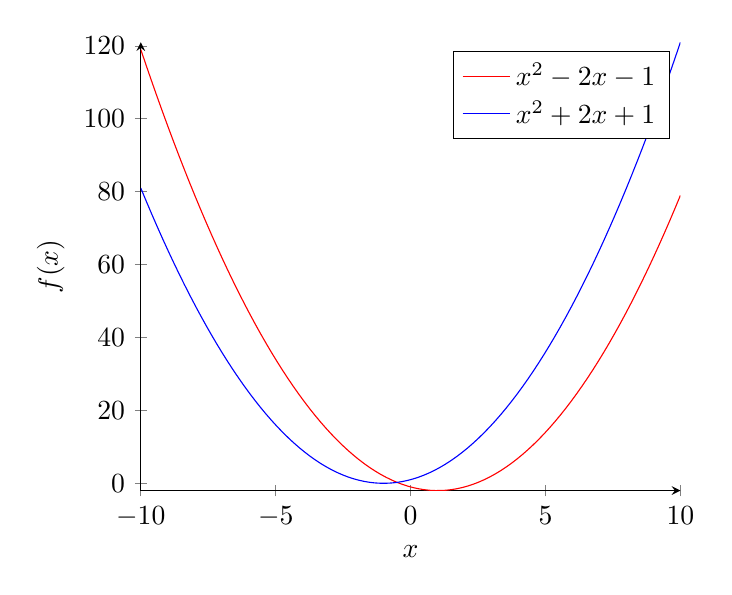
\begin{tikzpicture}
\begin{axis}[
    axis lines = left,
    xlabel = \(x\),
    ylabel = {\(f(x)\)},
]
%Below the red parabola is defined
\addplot [
    domain=-10:10, 
    samples=100, 
    color=red,
]
{x^2 - 2*x - 1};
\addlegendentry{\(x^2 - 2x - 1\)}
%Here the blue parabola is defined
\addplot [
    domain=-10:10, 
    samples=100, 
    color=blue,
    ]
    {x^2 + 2*x + 1};
\addlegendentry{\(x^2 + 2x + 1\)}

\end{axis}
\end{tikzpicture}

\vspace{1cm}
\section{Graph 3}

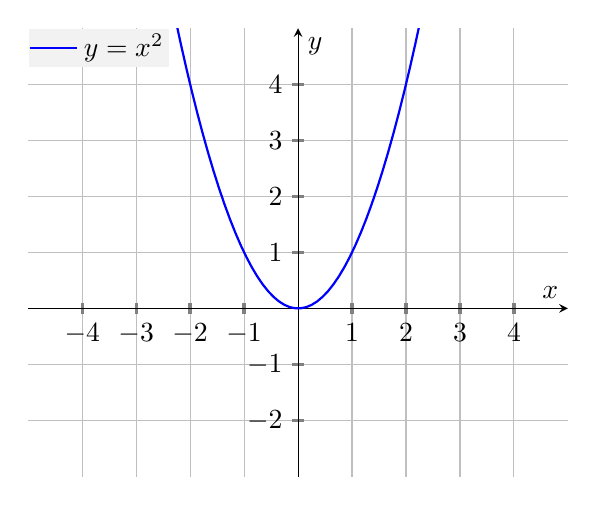
\begin{tikzpicture}
\begin{axis}[
  axis lines=middle,
  grid=major,
  xmin=-5,
  xmax=5,
  ymin=-3,
  ymax=5,
  xlabel=$x$,
  ylabel=$y$,
  xtick={-4,-3,...,4},
  ytick={-2,-1,...,4},
  tick style={very thick},
  legend style={
  at={(rel axis cs:0,1)},
  anchor=north west,draw=none,inner sep=0pt,fill=gray!10}
]
\addplot[blue,thick,samples=100] {x^2};
\addlegendentry{$y=x^2$}
\end{axis}
\end{tikzpicture}

\vspace{1cm}
\section{Blank graph 1}

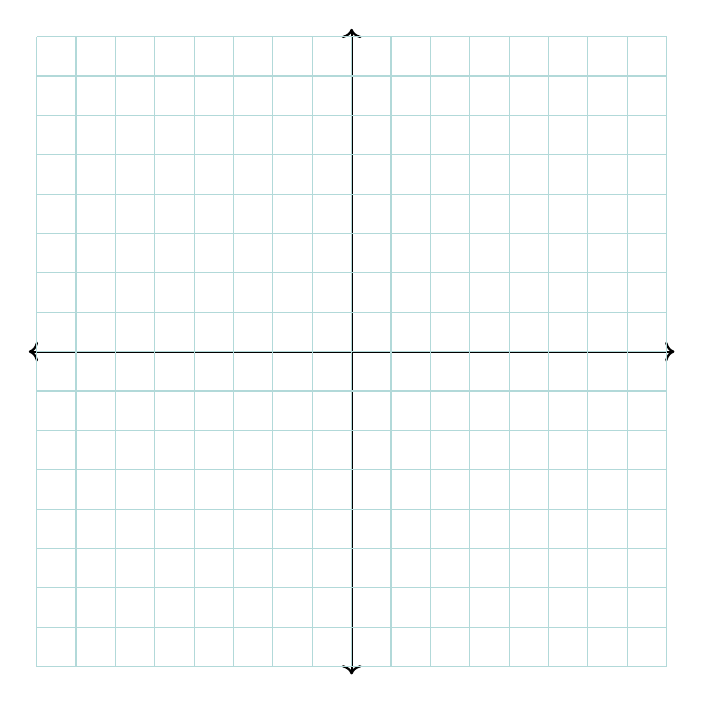
\begin{tikzpicture}
  % axis
  \draw[thick, <->] (0, -4.1) -- (0, 4.1);
  \draw[thick, <->] (-4.1, 0) -- (4.1, 0);

  % grid
  \draw[help lines, step = 0.5cm] (-4, -4) grid (4, 4);
\end{tikzpicture}

\vspace{1cm}
\section{Many Graphs}
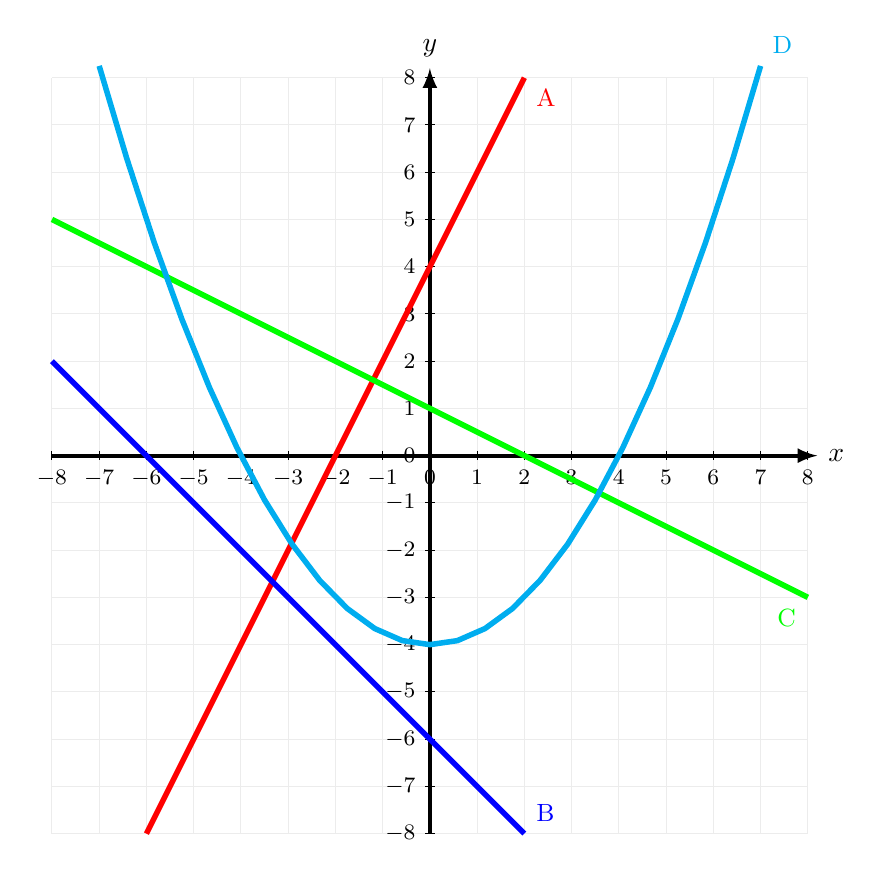
\begin{tikzpicture}[scale=0.60]
        \draw[gray!15,step=1cm] (-8,-8) grid (8,8);
        \draw[line width=0.5mm, -latex] (-8,0) -- (8.2,0) node[right] {$x$};
        \foreach \x in {-8,...,8} \draw (\x,.1)--(\x,-.1) node[below] {\footnotesize $\x$};
        \draw[line width=0.5mm,  -latex] (0,-8) -- (0,8.2) node[above] {$y$};
        \foreach \y in {-8,...,8} \draw (.1,\y)--(-.1,\y) node[left] {\footnotesize $\y$};

        % Red line with label 'a'
        \draw[red,line width=2pt] plot[domain= -6:2] (\x,{2*\x+4}) node[below right, font=\small] {A};
        % Blue line with label 'b'
        \draw[blue,line width=2pt] plot[domain= -8:2] (\x,{-1*\x-6}) node[above right, font=\small] {B};
        % Green line with label 'c'
        \draw[green,line width=2pt] plot[domain= -8:8] (\x,{-0.5*\x+1}) node[below left, font=\small] {C};
        % Cyan line with label 'd'
        \draw[cyan,line width=2pt] plot[domain= -7:7] (\x,{0.25*\x*\x-4}) node[above right, font=\small] {D};
    \end{tikzpicture}

\vspace{1cm}
\section{Blank Graph 2}
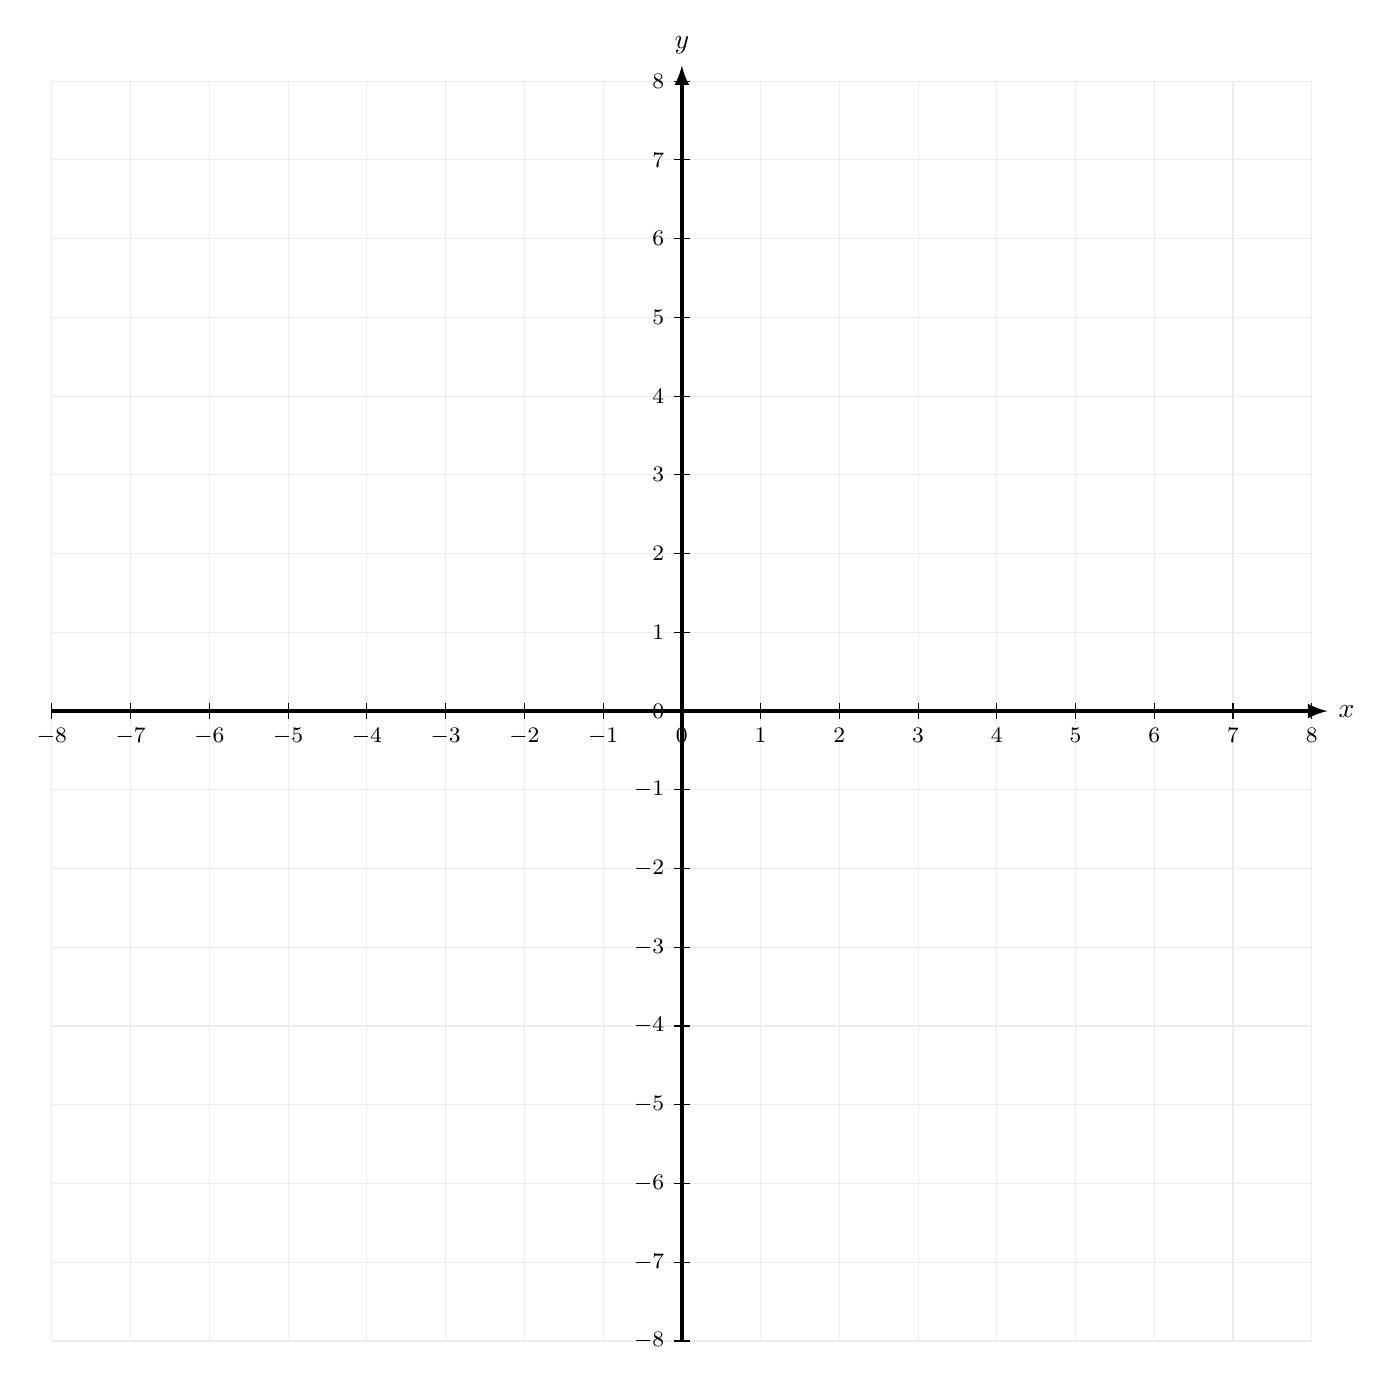
\begin{tikzpicture}
        \draw[gray!15,step=1cm] (-8,-8) grid (8,8);    
        \draw[line width=0.5mm, -latex] (-8,0) -- (8.2,0) node[right] {$x$};
        \foreach \x in {-8,...,8} \draw (\x,.1)--(\x,-.1) node[below] {\footnotesize $\x$};
        \draw[line width=0.5mm,  -latex] (0,-8) -- (0,8.2) node[above] {$y$};
        \foreach \y in {-8,...,8} \draw (.1,\y)--(-.1,\y) node[left] {\footnotesize $\y$};
        
\end{tikzpicture}

\vspace{1cm}
\section{Vector Graphs}
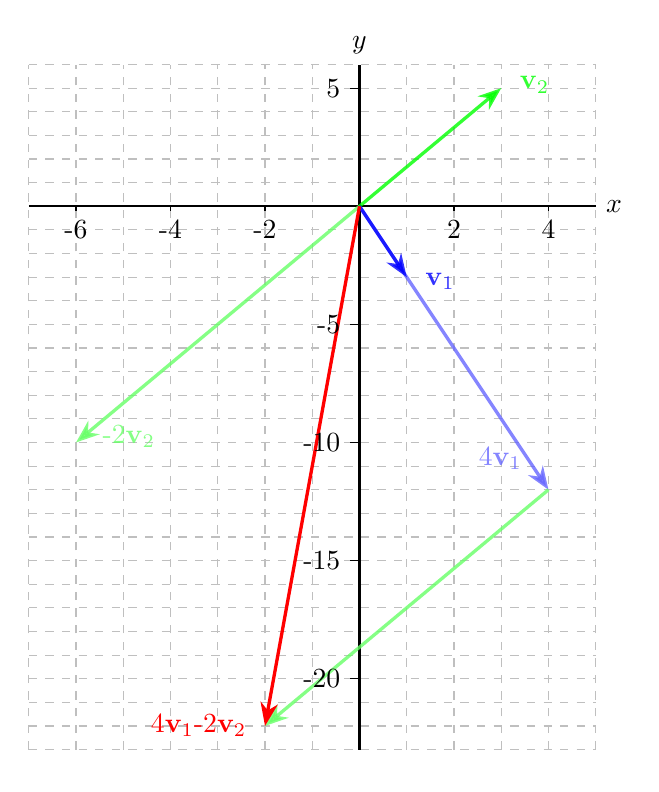
\begin{tikzpicture}
			[
				xscale=0.6,
				yscale=0.3,
				>=Stealth,
				grid style/.style={dashed, gray, opacity=0.5},
				axis style/.style={black, thick},
				vector style/.style={->, very thick}
			]
		% Draw the grid and axes
		\draw[grid style] (-7,-23) grid (5,6);
		\draw[axis style] (-7,0) -- (5,0) node[right] {$x$};
		\draw[axis style] (0,-23) -- (0,6) node[above] {$y$};

		% Draw the original vectors (lighter color)
		\draw[vector style, color=blue!60, opacity=0.8] (0,0) -- (4,-12) node[left, xshift=-2mm,yshift=4mm] {$4\mathbf{v}_1$};

		\draw[vector style, green, opacity=0.8] (0,0) -- (3,5) node[above right, xshift=1mm, yshift=-2mm] {$\mathbf{v}_2$};

		% Draw the scaled vectors (darker color)
		\draw[vector style, blue, opacity=0.8] (0,0) -- (1,-3) node[above right, xshift=1mm, yshift=-3mm] {$\mathbf{v}_1$};
		\draw[vector style, color=green!60, opacity=0.8] (0,0) -- (-6,-10) node[above right, xshift=2mm, yshift=-2mm] {-2$\mathbf{v}_2$};

		% Draw the head-to-tail vector addition (dashed line)
		\draw[vector style, color=green!60, opacity=0.8] (4,-12) -- (-2,-22) node[above left, yshift=-5mm] {};

		% Draw the resultant vector (red)
		\draw[vector style, red, very thick] (0,0) -- (-2,-22) node[left, xshift=-1mm] {4$\mathbf{v}_1$-2$\mathbf{v}_2$};

		% Add labels for coordinates
		\foreach \x in {-6,-4,-2,2,4}
			\draw (\x,0) -- (\x,-0.2) node[below] {\x};
		\foreach \y in {-20,-15,-10,-5,5}
			\draw (0,\y) -- (-0.2,\y) node[left] {\y};

		\end{tikzpicture}

\vspace{1cm}
\section{Simple Table}
\begin{center}
    \begin{tabular}{|c|c|c|c|c|c|c|c|}
        \hline
        Seconds & 0 & 1 & 2 & 3 & 4 & 5 & 6 \\
        \hline
        Feet & 6 & 8 & 10 & 12 & 14 & 16 & 18 \\
        \hline
    \end{tabular}
\end{center}

\vspace{8cm}
\section{Inserting Image}
Here is a picture of a cat, scaled to 50\% of its original size.

\begin{figure}[h!]
    \centering
    
\includegraphics[scale=0.5]{cat_picture2.png} % Change the filename here
    \caption{A cute cat}
    \label{fig:cat}
\end{figure}

The cat in Figure \ref{fig:cat} is very cute.
\end{document}

